\subsection{Composite Trapezoidal and Simpson's Rule}



\frame{
\begin{block}{}
An intuitive method\footnote{直观的方法} of finding the area under the curve $y = f(x)$ over $[a, b]$ is by approximating that area with a series of trapezoids that lie above the intervals $\{ [ x_k, x_{k+1} ] \}$. 
\end{block}
}

\frame{
\begin{block}{Theorem 5.2 (Composite Trapezoidal Rule).}
Suppose that the interval $[a, b]$ is subdivided into $M$ subintervals $[x_k, x_{k+1}]$ of width $h = (b - a)/M$ by using the 
equally spaced nodes $x_k = a + kh$, for $k = 0,1, \ldots, M$. 
The {\Large composite trapezoidal rule for $M$ subintervals} can be expressed in any of three equivalent ways:
\begin{equation*}
T (f, h) = \frac{h}{2} \sum_{k=1}^M \left( f(x_{k-1}) + f(x_k) \right) 
\end{equation*}
or 
\begin{equation*}
T (f, h) = \frac{h}{2} \left( f_0 + 2f_1 + 2f_2 + 2f_3 + \cdots + 2f_{M-2} + 2f_{M-1} + f_M \right) 
\end{equation*}
or 
\begin{equation*}
T (f, h) = \frac{h}{2} \left( f(a) + f(b) \right) + h \sum_{k=1}^{M-1}  f(x_k)
\end{equation*}
\end{block}
}


\frame{
\begin{block}{This is an approximation to the integral of $f(x)$ over $[a, b]$, and we write }
\begin{equation*}
\int_a^b f(x) dx \approx T(f, h)
\end{equation*}
\end{block}
}

\frame{
\frametitle{Proof of Theorem 5.2}
Apply the trapezoidal rule over each subinterval $[x_{k-1}, x_k]$ \footnote{(see Figure 5.6) in the textbook}.\\
Use the additive property of the integral for subintervals:
\begin{equation*}
\int_a^b f(x) dx = \sum_{k=1}^M \int_{x_{k-1}}^{x_k} f(x) dx \approx \sum_{k=1}^M \frac{h}{2} \left( f(x_{k-1}) + f(x_k) \right)
\end{equation*}
%\begin{figure}
%\begin{center}
%\includegraphics[width=110mm]{fig/ch-5/theorem_5-2_proof.png}
%\end{center}
%\end{figure}
\begin{figure}
\begin{center}
%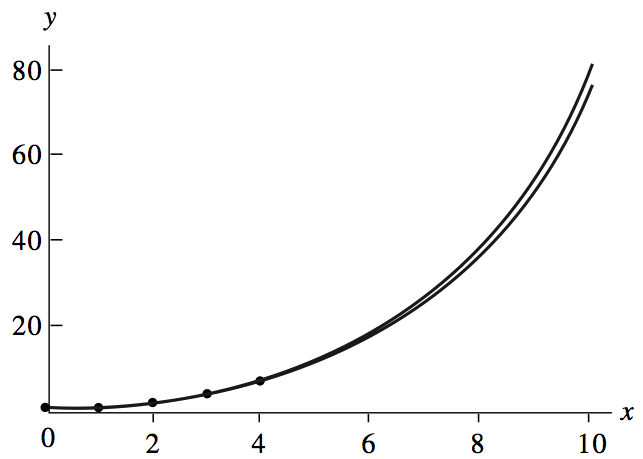
\includegraphics[width=80mm]{fig/ch-5/fig_5-6.png}
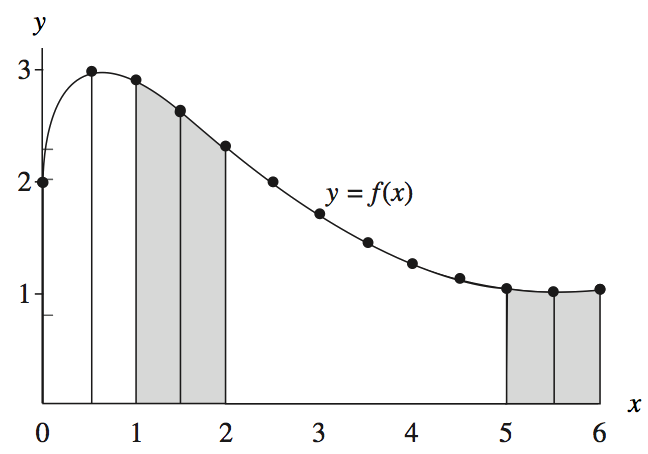
\includegraphics[width=50mm]{chap-5/fig_7-6.png} \\
Approximating $f(x) = 2 + sin(2\sqrt{x})$ with piecewise linear polynomials results in places where the approximation is close and places. 
\end{center}
\end{figure}
}

%\frame{
%Since $h \slash 2$ is a constant, the distributive law of addition can be applied to obtain (1a). 
%Formula (1b) is the expanded version of (1a). 
%Formula (1c) shows how to group all the intermediate terms in (1b) that are multiplied by 2.
%}

\frame{
\begin{block}{}
{\Huge To achieve accuracy, the composite trapezoidal rule must be applied with many subintervals.}
\end{block}
%\begin{itemize}
%\item Approximating $f(x) = 2 + sin(2\sqrt{x})$ with piecewise linear polynomials results in places where the approximation is close and places where it is not. 
%\vspece{0.3cm}
%\item To achieve accuracy, the composite trapezoidal rule must be applied with many subintervals. 
%\vspece{0.3cm}
%\item In the next example we have chosen to integrate this function numerically over the interval $[1,6]$. 
%\vspece{0.3cm}
%\item Investigation of the integral over $[0,1]$ is left as an exercise. 
%\end{itemize}
}

\frame{
\begin{block}{Example 5.5.}
Consider $f (x) = 2 + sin(2\sqrt{x}$. 
Use the composite trapezoidal rule with $11$ sample points to compute an approximation to the integral of $f (x)$ taken over $[1, 6]$.
\end{block}
To generate $11$ sample points, we use $M = 10$ and $h = (6 - 1) \slash 10 = 1 \slash 2$. 
Using the formula , the computation is
\begin{equation*}
\begin{array}{l l}
T \left( f, \frac{1}{2} \right) & = \frac{1\slash 2}{2} \left( f(1) + f(6) \right) \\
& + \frac{1}{2} \left( f(\frac{3}{2}) + f(2) + f(\frac{5}{2}) + f(3) + f(\frac{7}{2}) + f(4) + f(\frac{9}{2}) + f(5) + f(\frac{11}{2}) \right) \\
& \\
& = \frac{1}{4}  (2.90929743 + 1.01735756) \\
& + \frac{1}{2} (2.63815764 + 2.30807174 + 1.97931647 + 1.68305284 \\
&  + 1.43530410 + 1.24319750 + 1.10831775 + 1.02872220  \\
& + 1.00024140 ) \\
& \\
& =  \frac{1}{4} (3.92665499) + \frac{1}{2} (14.42438165) \\
%& \\
& = 0.98166375 + 7.21219083 = 8.19385457.
\end{array}
\end{equation*}
%\begin{figure}
%\begin{center}
%\includegraphics[width=110mm]{fig/ch-5/ex_5-5.png}
%\end{center}
%\end{figure}
}

\frame{
\begin{block}{Theorem 5.3 (Composite Simpson Rule).}	
Suppose that $[a,b]$ is subdivided into $2M$ subintervals $[x_k,x_{k+1}]$ of equal width $h=(b-a) \slash (2M)$ by using $x_k = a + kh$ for $k = 0, 1, \ldots, 2 M$. 
The {\Large composite Simpson rule} for $2 M$ subintervals can be expressed in any of three equivalent ways:
\begin{equation*}
S(f, h) = \frac{h}{3} \sum_{k=1}^M \left(  f(x_{2k-2}) + 4 f(x_{2k-1}) + f(x_{2k}) \right)
\end{equation*}
or
\begin{equation*}
\begin{array}{l l}
S(f, h) & = \frac{h}{3}  ( f_0 + 4 f_1 + 2 f_2 + 4 f_3 \\
& + \cdots + 2 f_{2M-2} + 4 f_{2M-1} + f_{2M})
\end{array}
\end{equation*}
or
\begin{equation*}
S(f, h) = \frac{h}{3} \left( f(a) + f(b) \right) +  \frac{2h}{3} \sum_{k=1}^{M-1}f(x_{2k}) + \frac{4h}{3} \sum_{k=1}^{M-1}f(x_{2k-1})
\end{equation*}
\end{block}
%\begin{figure}
%\begin{center}
%\includegraphics[width=110mm]{fig/ch-5/theorem_5-3.png}
%\end{center}
%\end{figure}
}

\frame{
\begin{block}{This is an approximation to the integral of $f(x)$ over $[a, b]$, and we write }
\begin{equation*}
\int_a^b f(x) dx \approx S(f, h)
\end{equation*}
\end{block}
}

\frame{
\frametitle{Proof of Theorem 5.3.}
Apply Simpson’s rule over each subinterval $[x_{2k-2}, x_{2k} ]$\footnote{see Figure 5.7 in textbook}. 
Use the additive property of the integral for subintervals :
\begin{equation*}
\begin{array}{l l}
\int_a^b f(x) dx & = \sum_{k=1}^M \int_{x_{2k-2}}^{x_{2k}} f(x) dx \\
& \approx \sum_{k=1}^M \frac{h}{3} \left( f(x_{2k-2}) + 4f(x_{2k-1}) + f(x_{2k}) \right)
\end{array}
\end{equation*}
%\begin{figure}
%\begin{center}
%\includegraphics[width=110mm]{fig/ch-5/theorem_5-3_proof.png}
%\end{center}
%\end{figure}
%\begin{itemize}
%\item Since $h/3$ is a constant, the distributive law of addition can be applied to obtain (5.24). 
%\item Formula (5.25) is the expanded version of (5.24).
%\item Formula (5.26) groups all the intermediate terms in (5.25) that are multiplied by $2$ and those that are multiplied by $4$ .
%\end{itemize}
\begin{figure}
\begin{center}
%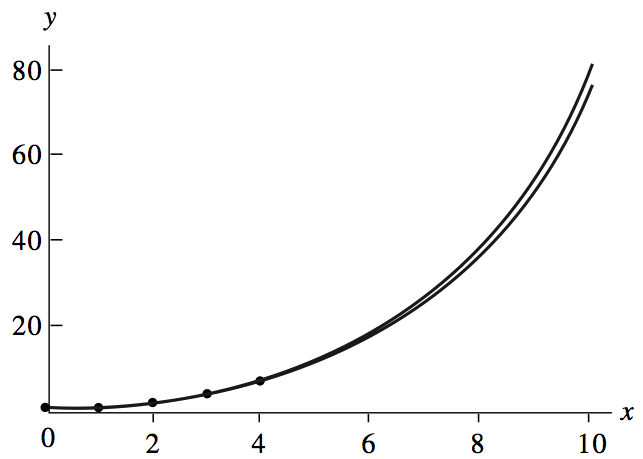
\includegraphics[width=80mm]{fig/ch-5/fig_5-6.png}
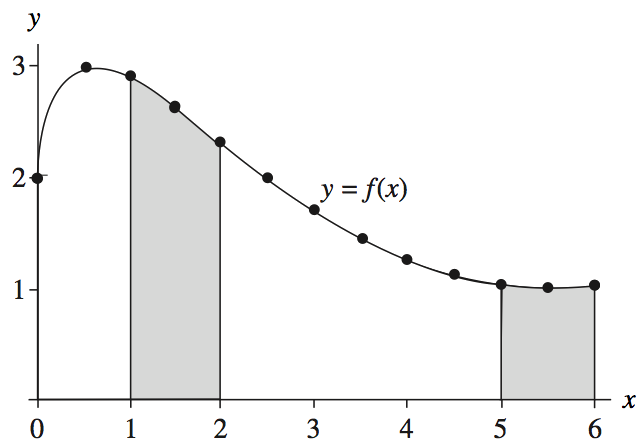
\includegraphics[width=50mm]{chap-5/fig_7-7.png} \\
Approximating $f(x) = 2 + sin(2\sqrt{x})$ with piecewise linear polynomials results in places where the approximation is close and places where it is not. 
\end{center}
\end{figure}
}

%\frame{
%\begin{figure}
%\begin{center}
%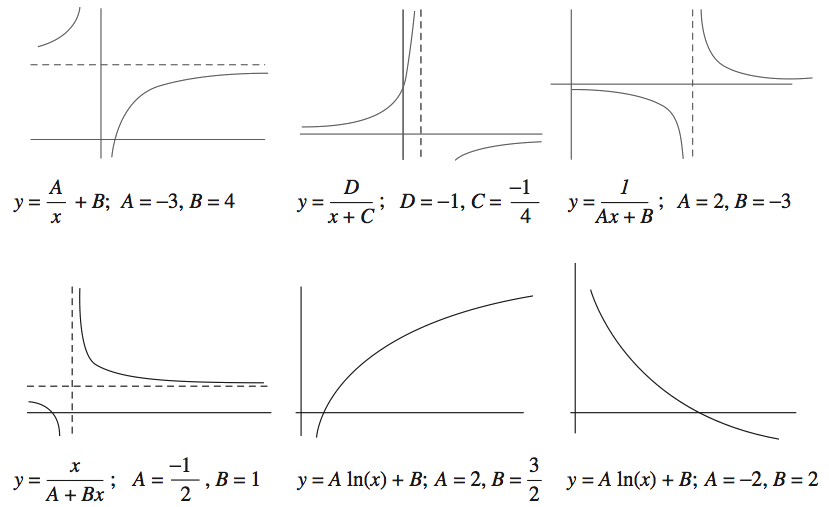
\includegraphics[width=110mm]{fig/ch-5/fig_5-7.png}
%\end{center}
%\end{figure}
%}

%\frame{
%\begin{itemize}
%\item Approximating $f(x) = 2 + \sin(2\sqrt{x})$ with piecewise quadratic polynomials produces places where the approximation is close and places where it is not. 
%\item To achieve accuracy the composite Simpson rule must be applied with several subintervals. 
%\item In the next example we have chosen to integrate this function numerically over $[1,6]$ and leave investigation of the integral over $[0,1]$ as an exercise. 
%\end{itemize}
%}

\frame{
\begin{block}{Example 5.6.}
Consider $f (x) = 2 + sin(2\sqrt{x})$. 
Use the composite Simpson rule with $11$ sample points to compute an approximation to the integral of $f (x )$ taken over $[1, 6]$.
\end{block}
To generate $11$ sample points, we must use $M = 5$ and $h = (6 - 1) \slash 10 = 1 \slash 2$. 
Using the formula, the computation is
\begin{equation*}
\begin{array}{l l}
S(f,\frac{1}{2}) & = \frac{1}{6} \left( f(1) + f(6) \right) + \frac{1}{3} \left( f (2) + f (3) + f (4) + f (5) \right) \\
& + \frac{2}{3} \left( f(\frac{3}{2})+ f(\frac{5}{2})+ f(\frac{7}{2})+ f(\frac{9}{2})+ f(\frac{11}{2}) \right) \\
& \\
& =  \frac{1}{6} (2.90929743 + 1.01735756) \\
& + \frac{1}{3} (2.30807174 + 1.68305284 + 1.24319750 + 1.02872220) \\
& + \frac{2}{3}  (2.63815764 + 1.97931647 + 1.43530410 + 1.10831775 \\
& + 1.00024140) \\
& \\
& =  0.65444250 + 2.08768143 + 5.44089157 = 8.18301550.
\end{array}
\end{equation*}
%\begin{figure}
%\begin{center}
%\includegraphics[width=110mm]{fig/ch-5/ex_5-6.png}
%\end{center}
%\end{figure}
}

\frame{
\frametitle{Error Analysis }
\begin{itemize}
\item The significance of the next two results is to understand that the error terms $E_T(f, h)$ and $E_S(f, h)$ for the composite trapezoidal rule and composite Simpson rule are of the order $O(h^2)$ and $O(h^4)$, respectively. 
\vspace{0.3cm}
\item This shows that the error for Simpson's rule converges to zero faster than the error for the trapezoidal rule as the step size h decreases to zero. 
\vspace{0.3cm}
\item In cases where the derivatives of $f(x)$ are known, the formulas 
\begin{equation*}
E_T(f, h) = \frac{-(b-a)f^{(2)}(c)h^2}{12} \ \ and \ \ E_S(f, h) = \frac{-(b-a)f^{(4)}h^4}{180}
\end{equation*}
can be used to estimate the number of subintervals required to achieve a specified accuracy.
\end{itemize}
%\begin{figure}
%\begin{center}
%\includegraphics[width=100mm]{fig/ch-5/p_215.png}
%\end{center}
%\end{figure}
}

\frame{
\begin{block}{Corollary 5.2 (Trapezoidal Rule: Error Analysis).}
Suppose that $[a, b]$ is subdivided into $M$ subintervals $[x_k, x_{k+1}]$ of width $h = (b - a) \slash M$. 
The composite trapezoidal rule
\begin{equation*}
T (f, h) = \frac{h}{2} (f(a) + f(b)) + h \sum_{k=1}^{M-1} f(x_k)
\end{equation*}
is an approximation to the integral
\begin{equation*}
\int_a^b f(x) dx = T (f, h) + E_T(f, h)
\end{equation*}
%\begin{figure}
%\begin{center}
%\includegraphics[width=110mm]{fig/ch-5/coro_5-2.png}
%\end{center}
%\end{figure}
%\begin{figure}
%\begin{center}
%\includegraphics[width=110mm]{fig/ch-5/coro_5-2_2.png}
%\end{center}
%\end{figure}
Furthermore, if $f \in C^2[a, b]$, there exists a value $c$ with $a < c < b$ so that the error term $E_T (f, h)$ has the form 
\begin{equation*}
E_T (f, h) = \frac{-(b-a)f^{(2)}(c)h^2}{12} = O(h^2)
\end{equation*}
\end{block}
}

\frame{
\frametitle{Proof. of Corollary 5.2} 
We first determine the error term when the rule is applied over $[x_0, x_1]$. 
Integrating the Lagrange polynomial $P_1(x)$ and its remainder yields
\begin{equation*}
\int_{x_0}^{x_1} f(x) dx = \int_{x_0}^{x_1} P_1(x) dx + \int_{x_0}^{x_1} \frac{(x-x_0)(x-x_1)f^{(2)}(c(x))}{2!} dx
\end{equation*}
The term $(x - x_0)(x - x_1)$ does not change sign on $[x_0, x_1]$, and $f^{(2)}(c(x))$ is continuous. 

Hence the second mean value theorem for integrals implies that there exists a value $c_1$ so that
\begin{equation*}
\int_{x_0}^{x_1} f(x) dx = \frac{h}{2}(f_0+f_1) + f^{(2)}(c_1) \int_{x_0}^{x_1} \frac{(x-x_0)(x-x_1)}{2!} dx
\end{equation*}
}

\frame{
Use the change of variable $x = x_0 + ht$ in the integral on the right side of above equation :
\begin{equation*}
\begin{array}{l l}
\int_{x_0}^{x_1} f(x) dx & = \frac{h}{2} (f_0+f_1) + \frac{f^{(2)}(c_1)}{2} \int_0^1 h(t-0)h(t-1) dt \\
& \\
& = \frac{h}{2}(f_0 + f_1) + \frac{f^{(2)}(c_1)h^3}{2} \int_0^1 (t^2-t) dt \\
& \\
& = \frac{h}{2}(f_0 + f_1) + \frac{f^{(2)}(c_1)h^3}{12}
\end{array}
\end{equation*}
}

\frame{
Now we are ready to add up the error terms for all of the intervals$ [x_k, x_{k+1}]$: 
\begin{equation*}
\begin{array}{l l}
\int_{x_0}^{x_1} f(x) dx & = \sum_{k=1}^M \int_{x_{k-1}}^{x_k} f(x) dx \\
& = \sum_{k=1}^M \frac{h}{2} (f(x_{k-1})+f(x_k)) - \frac{h^3}{12} \sum_{k=1}^M f^{(2)}(c_k)
\end{array}
\end{equation*}
\begin{itemize}
\item The first sum is the composite trapezoidal rule $T(f, h)$.  
\item In the second term, one factor of $h$ is replaced with its equivalent $h = (b - a) \slash M$, and the result is 
\begin{equation*}
\int_a^b f(x) dx = T(f, h) - \frac{(b-a) h^2}{12} \left( \frac{1}{M} \sum_{k=1}^M f^{(2)} (c_k) \right)
\end{equation*}
\end{itemize}
}

\frame{
The term in parentheses can be recognized as an average of values for the second derivative and hence is replaced by $f^{(2)}(c)$. 
Therefore, we have established that 
\begin{equation*}
\int_a^b f(x) dx = T(f, h) - \frac{(b-a) f^{(2)} (c) h^2 }{12} 
\end{equation*}
and the proof of Corollary 5.2 is complete. 
}

\frame{
\begin{block}{Corollary 5.3 (Simpson’s Rule: Error Analysis).}
Suppose that $[a, b]$ is subdivided into $2M$ subintervals $[x_k, x_{k+1}]$ of equal width $h = (b - a) \slash (2M)$. 
The composite Simpson rule 
\begin{equation*}
S(f, h) = \frac{h}{3} ( f(a) + f(b) ) + \frac{2h}{3} \sum_{k=1}^{M-1} f(x_{2k}) + \frac{4h}{3} \sum_{k=1}^M f(x_{2k-1})
\end{equation*}
is an approximation to the integral
\begin{equation*}
\int_a^b f(x) dx = S(f, h) + E_s(f,h)
\end{equation*}
Furthermore, if  $f \in C^4[a,b]$, there exists a value $c$ with $a < c < b$ so that the error term $E_S(f, h)$ has the form
\begin{equation*}
E_S(f, h) = \frac{-(b-a)f^{(4)}(c)h^4}{180} = O(h^4)
\end{equation*}
\end{block}
}

\frame{
\begin{block}{Example 5.7.}
Consider $f (x) = 2 + sin(2\sqrt{x})$. 
Investigate the error when the composite trapezoidal rule is used over $[1, 6]$ and the number of subintervals is $10$, $20$, $40$, $80$, and $160$.
\end{block}
\begin{figure}
\begin{center}
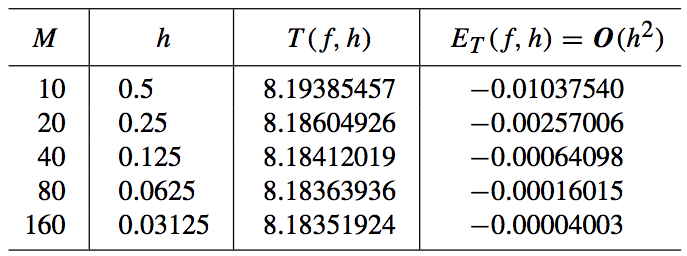
\includegraphics[width=60mm]{chap-5/tab_7-2.png}
\end{center}
\end{figure}
The above table 5.2 shows the approximations $T (f, h)$. 
The antiderivative of $f (x)$ is
\begin{equation*}
F(x) = 2x - \sqrt{x} \cos ( 2\sqrt{x}) + \frac{\sin(2\sqrt{x})}{2}
\end{equation*}
and the true value of the  definite integral is
\begin{equation*}
\int_1^6 f(x)dx = \left. F(x)  \right|_{x=1}^{x=6} = 8.1834792007
\end{equation*}
}

%\frame{
%This value was used to compute the values $E_T(f, h) = 8.1834792077 - T(f, h)$ in Table 5.2. 
%It is important to observe that when $h$ is reduced by a factor of $\frac{1}{2}$ the successive errors $E_T(f, h)$ are diminished by approximately $\frac{1}{4}$. 
%This confirms that the order is $O( h^2)$. 
%\begin{figure}
%\begin{center}
%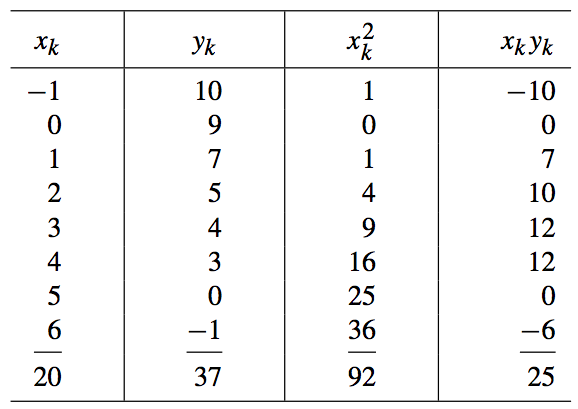
\includegraphics[width=90mm]{fig/ch-5/tab_5-2.png}
%\end{center}
%\end{figure}
%}

\frame{ 
\begin{block}{Example 5.8.}
Consider $f(x) = 2 + sin(2\sqrt{x})$. 
Investigate the error when the composite Simpson rule is used over $[1,6]$ and the number of subintervals is $10$, $20$, $40$, $80$, and $160$. 
\end{block}
\begin{itemize}
\item The following table\footnote{Table 5.3 in textbook}  shows the approximations $S(f, h)$. 
\item The true value of the integral is $8.1834792077$, which was used to compute the values $E_S(f, h) = 8.1834792077 - S(f, h)$ in the Table. 
\item It is important to observe that when $h$ is reduced by a factor of $\frac{1}{2}$, the successive errors $E_S(f, h)$ are diminished by approximately $\frac{1}{16}$. 
\item This confirms that the order is $O(h^4)$. 
\end{itemize}
%}

%\frame{
\begin{figure}
\begin{center}
%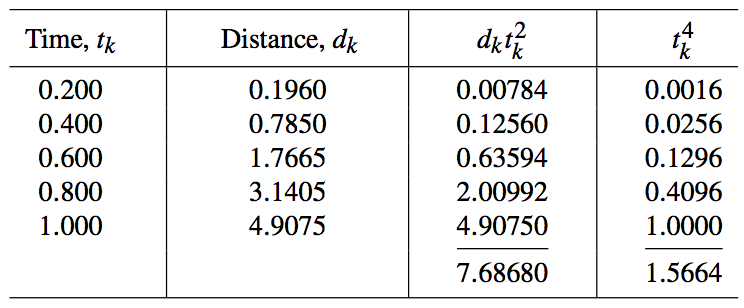
\includegraphics[width=90mm]{fig/ch-5/tab_5-3.png}
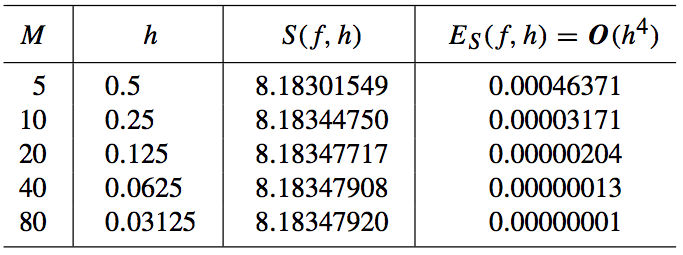
\includegraphics[width=60mm]{chap-5/tab_7-3.png}
\end{center}
\end{figure}
}

%\frame{
%\begin{figure}
%\begin{center}
%\includegraphics[width=110mm]{fig/ch-5/ex_5-9.png}
%\end{center}
%\end{figure}
%}

%\frame{
%\begin{itemize}
%\item Solving (5.41), we find that $22821.77 \le M$. 
%\item Since $M$ must be an integer, we choose $M = 22,822$, and the corresponding step size is $h = 5/22,822 = 0.000219086846$. 
%\item When the composite trapezoidal rule is implemented with this many function evaluations, there is a possibility  that the rounded-off function evaluations will produce a significant amount of error. 
%\item When the computation was performed, the result was 
%\end{itemize}
%\begin{figure}
%\begin{center}
%\includegraphics[width=75mm]{fig/ch-5/p_218.png}
%\end{center}
%\end{figure}
%which compares favorably with the true value $\int_2^7 \frac{dx}{x} = In (x)|_{x=2}^{x=7} = 1.252762968$.
%}

%\frame{
%The error is smaller than predicted because the bound $\frac{1}{4}$ for $|f"(c)|$ was used. \\
%Experimentation shows that it takes about $10,001$ function evaluations to achieve the desired accuracy of $5 \times 10^{-9}$, and when %the calculation is performed with $M = 10,000$, the result is 
%\begin{figure}
%\begin{center}
%\includegraphics[width=50mm]{fig/ch-5/p_218_2.png}
%\end{center}
%\end{figure}
%The composite trapezoidal rule usually requires a large number of function evaluations to achieve an accurate answer. \\
%This is contrasted in the next example with Simpson's rule, which will require significantly fewer evaluations. 
%}

%\frame{
%\begin{figure}
%\begin{center}
%\includegraphics[width=110mm]{fig/ch-5/ex_5-10.png}
%\end{center}
%\end{figure}
%}

%\frame{
%\begin{figure}
%\begin{center}
%\includegraphics[width=110mm]{fig/ch-5/ex_5-10_2.png}
%\end{center}
%\end{figure}
%}

%\frame{
%So we see that the composite' Simpson rule using $229$ evaluations of $f(x)$ and the composite trapezoidal rule using $22,823$ evaluations of $f(x)$ achieve the same accuracy.  \\
%In Example 5.10, Simpson's rule required about $\frac{1}{100}$ the number of function evaluations. 
%}

%\frame{
%\begin{figure}
%\begin{center}
%\includegraphics[width=110mm]{fig/ch-5/prog_5-1.png}
%\end{center}
%\end{figure}
%}

%\frame{
%\begin{figure}
%\begin{center}
%\includegraphics[width=110mm]{fig/ch-5/prog_5-2.png}
%\end{center}
%\end{figure}
%}
